\section{代理模型构建}\label{sec:surrogate}

\begin{chapterquestion}
\textbf{本章研究的问题}：代理模型的预测精度是否足以支撑后续优化？
\end{chapterquestion}

\subsection{模型选型}

为建立从工况参数到稳定性评分的回归映射，本文对 6 个模型做了系统对比；
模型对比仅用于确定代理模型的选择，不展开逐模型讨论。

\begin{table}[H]
\centering
\caption{6 模型性能对比（测试集）——选型依据}
\begin{tabular}{lrrrr}
\toprule
模型 & R$^2$ & MSE & 延迟 (ms) & 角色 \\
\midrule
M1 Ridge & 0.6330 & 225.00 & 0.034 & 线性基准（表明问题强非线性） \\
M2 RandomForest & 1.0000 & 0.0000 & 37.07 & 高精度但延迟高、无 $\sigma$ \\
M3 \textbf{XGBoost} & \textbf{0.9999} & \textbf{0.0312} & \textbf{0.242} & \textbf{选用：可解释性 + 算法公平比较} \\
M4 MLP & 0.9994 & 0.3897 & 0.403 & 神经网络基准 \\
M5 TabNet & 0.9997 & 0.2002 & 7.847 & 注意力表格模型 \\
M6 \textbf{DeepEnsemble} & 0.9995 & 0.3272 & 1.230 & \textbf{选用：提供不确定性 $\sigma(x)$} \\
\bottomrule
\end{tabular}
\label{tab:model_cmp}
\end{table}

\begin{figure}[H]
\centering
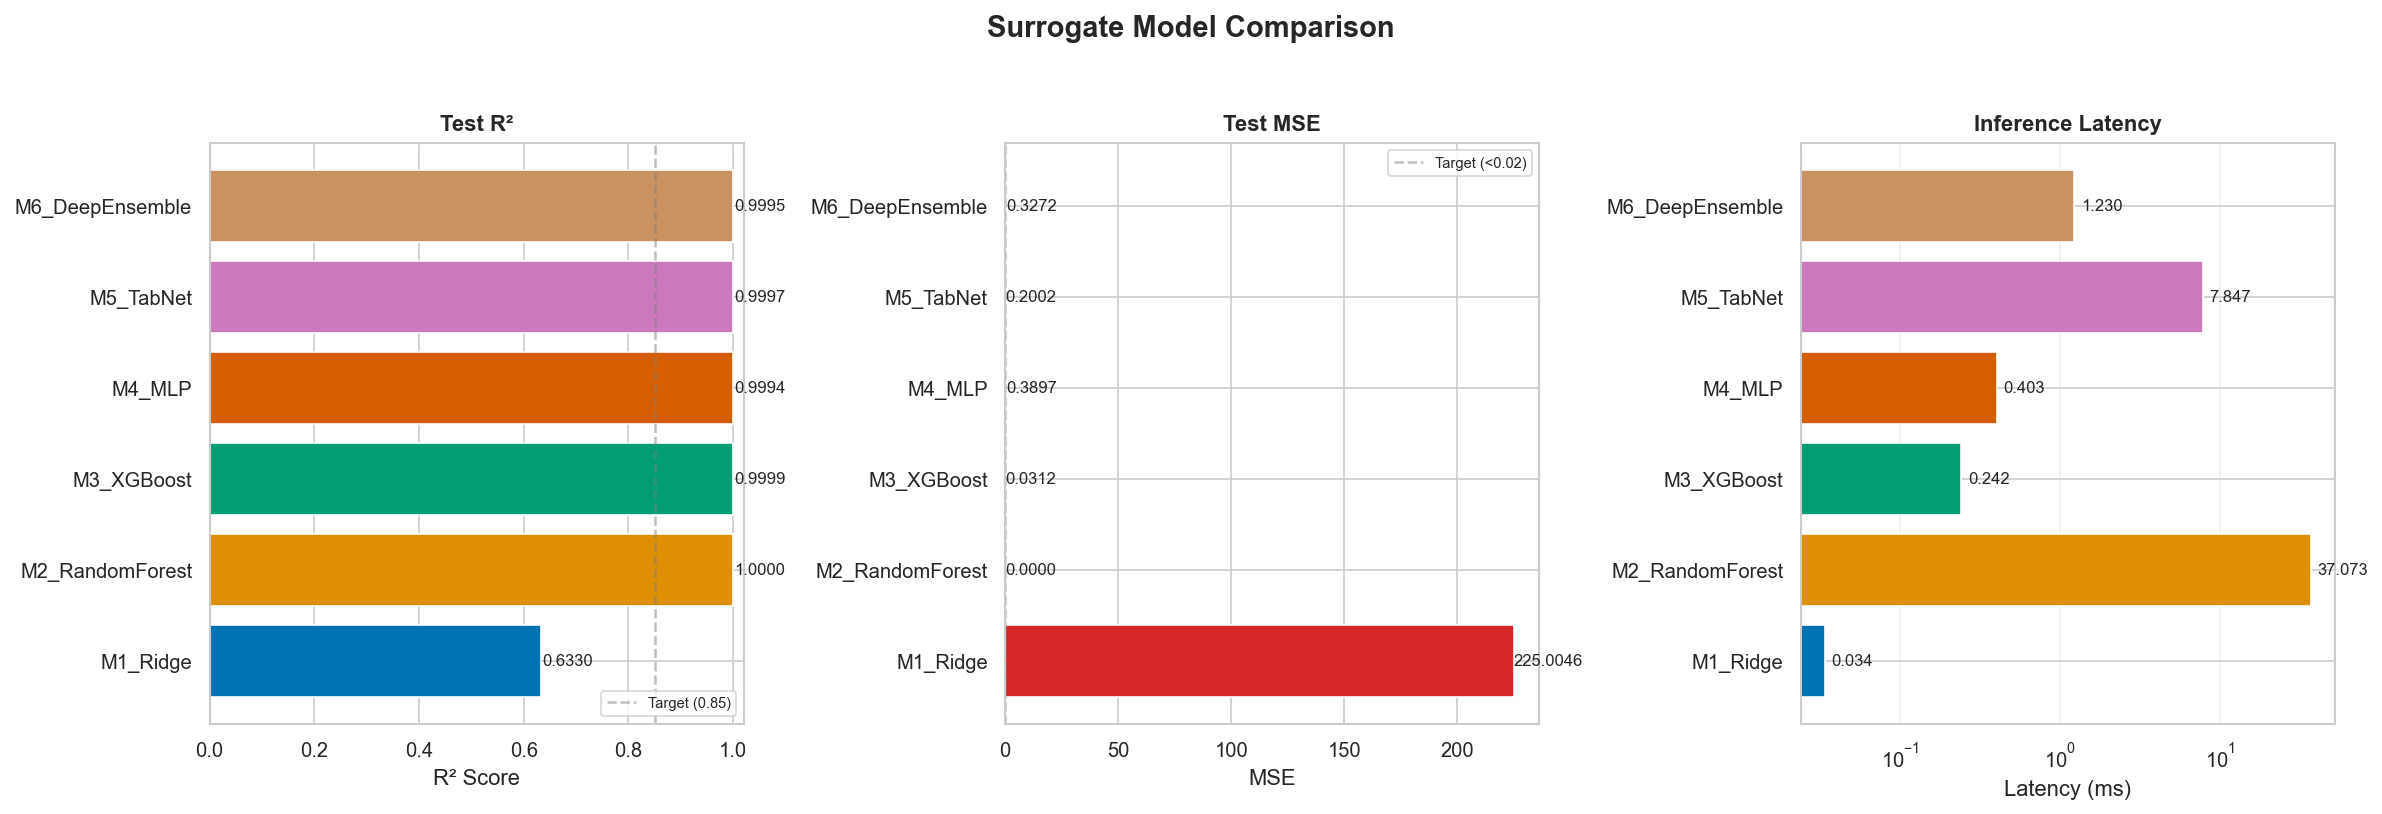
\includegraphics[width=0.78\textwidth]{figures/03_model_comparison.png}
\caption{6 模型性能对比可视化（R$^2$/MSE/MAE/延迟）}
\label{fig:model_cmp_fig}
\end{figure}

选型结论简单明了，并贯穿全文：
\textbf{XGBoost}（精度最高、延迟最低、TreeExplainer 原生支持）
用于可解释性分析与算法公平比较；
\textbf{DeepEnsemble}（3 个独立 MLP 的集成）用于风险敏感寻优，
因为只有它能输出预测均值 $\mu(x)$ 与成员间分歧 $\sigma(x)$——
后者是后续可信性分析所必需的信号。
开题设定的"BP 神经网络"因此退居为基准之一（M4），
体现数据驱动研究由证据而非预设决定选型的原则。

\subsection{关于 R$^2\approx 1$ 的说明}

代理精度逼近完美（RF 达 $R^2=1.0000$，XGBoost $0.9999$），初看异常。
结合第~\ref{sec:dataset}~节的数据来源可作如下解释：
数据由 XGBoost 引擎生成，本质是某经验模型的数值近似输出；
被测 XGBoost 与生成器共享架构与归纳偏置，能近乎复现生成规则是\emph{数学上可预期的}。
更说明问题的是：即便 Random Forest（基于 Bagging 与随机子空间，
架构与生成器不同）也能达到近零误差，
这表明\textbf{该数据生成机制本身具有极强的结构规律性}——
模型性能已逼近该数据集的信息上限，不同架构间的差异被压缩至极小。

5 折交叉验证进一步显示 XGBoost 各折 R$^2$ 标准差 $<0.0001$，泛化稳定。
但必须诚实指出：K-Fold 验证的是"训练-测试同分布"下的稳定性，
\emph{不能}排除生成器同源偏置或共享归纳偏置带来的结构优势。
换言之，这种"准"是相对于一个内部高度规律的合成世界而言的。

\textbf{同源数据风险}：数据由 XGBoost Generator 生成，而主代理同样采用 XGBoost，
二者构成"XGBoost 学习 XGBoost"的同源结构；因此 $R^2=0.9999$ 受同源偏置影响，
并不能充分说明代理具备对真实气动物理规律的泛化能力。
本文后续分析关注的是代理模型的优化行为与可信性问题，
而非其对真实气动物理规律的拟合能力。

\subsection{本阶段小结}

至此，代理模型构建阶段完成：已获得延迟亚毫秒、预测精度很高的代理模型。

需要指出，高精度度量的是\emph{在数据覆盖区域复现已知样本}的能力，
并不保证\emph{在优化器所探索的区域}同样可靠。
第~\ref{sec:anomaly}~节考察将该代理用于参数寻优时的表现。
